\documentclass[10pt,twocolumn]{article}

% use the oxycomps style file
\usepackage{oxycomps}
\usepackage{graphicx}
\usepackage{tabularx}

% usage: \fixme[comments describing issue]{text to be fixed}
% define \fixme as not doing anything special
\newcommand{\fixme}[2][]{#2}
% overwrite it so it shows up as red
\renewcommand{\fixme}[2][]{\textcolor{red}{#2}}
% overwrite it again so related text shows as footnotes
%\renewcommand{\fixme}[2][]{\textcolor{red}{#2\footnote{#1}}}

% read references.bib for the bibtex data
\bibliography{references}

% include metadata in the generated pdf file
\pdfinfo{
    /Title (Nodeaa: A Browser-Based Platform for Modular Sound Processing and Node-Based Audio Routing Using the WebAudio API)
    /Author (August Ross)
}

% set the title and author information
\title{Nodeaa: A Browser-Based Platform for Modular Sound Processing and Node-Based Audio Routing Using the WebAudio API}
\author{August Ross}
\affiliation{Occidental College}
\email{aross3@oxy.edu}

\begin{document}

\maketitle

\section{Introduction}

Digital Audio Workstations (DAWs) have long been essential tools for musicians, sound designers, and audio engineers. However, traditional DAWs are often limited by their dependency on specific operating systems, high system resource requirements, price, and the need for installation and maintenance. With the increasing prevalence of browser-based applications and the capabilities of the WebAudio API \cite{smus2013web}, the browser has emerged as a viable platform for real-time audio synthesis and manipulation. \textit{Nodeaa}, a modular sound processing and node-based dynamic audio routing tool, demonstrates the potential of the browser as a fully functional DAW. Inspired by established tools like MaxMSP and Pure Data, \textit{Nodeaa} enables users to create, manipulate, and route audio signals through an intuitive node-based interface, all within a web browser.

\begin{figure}[ht]
    \centering
    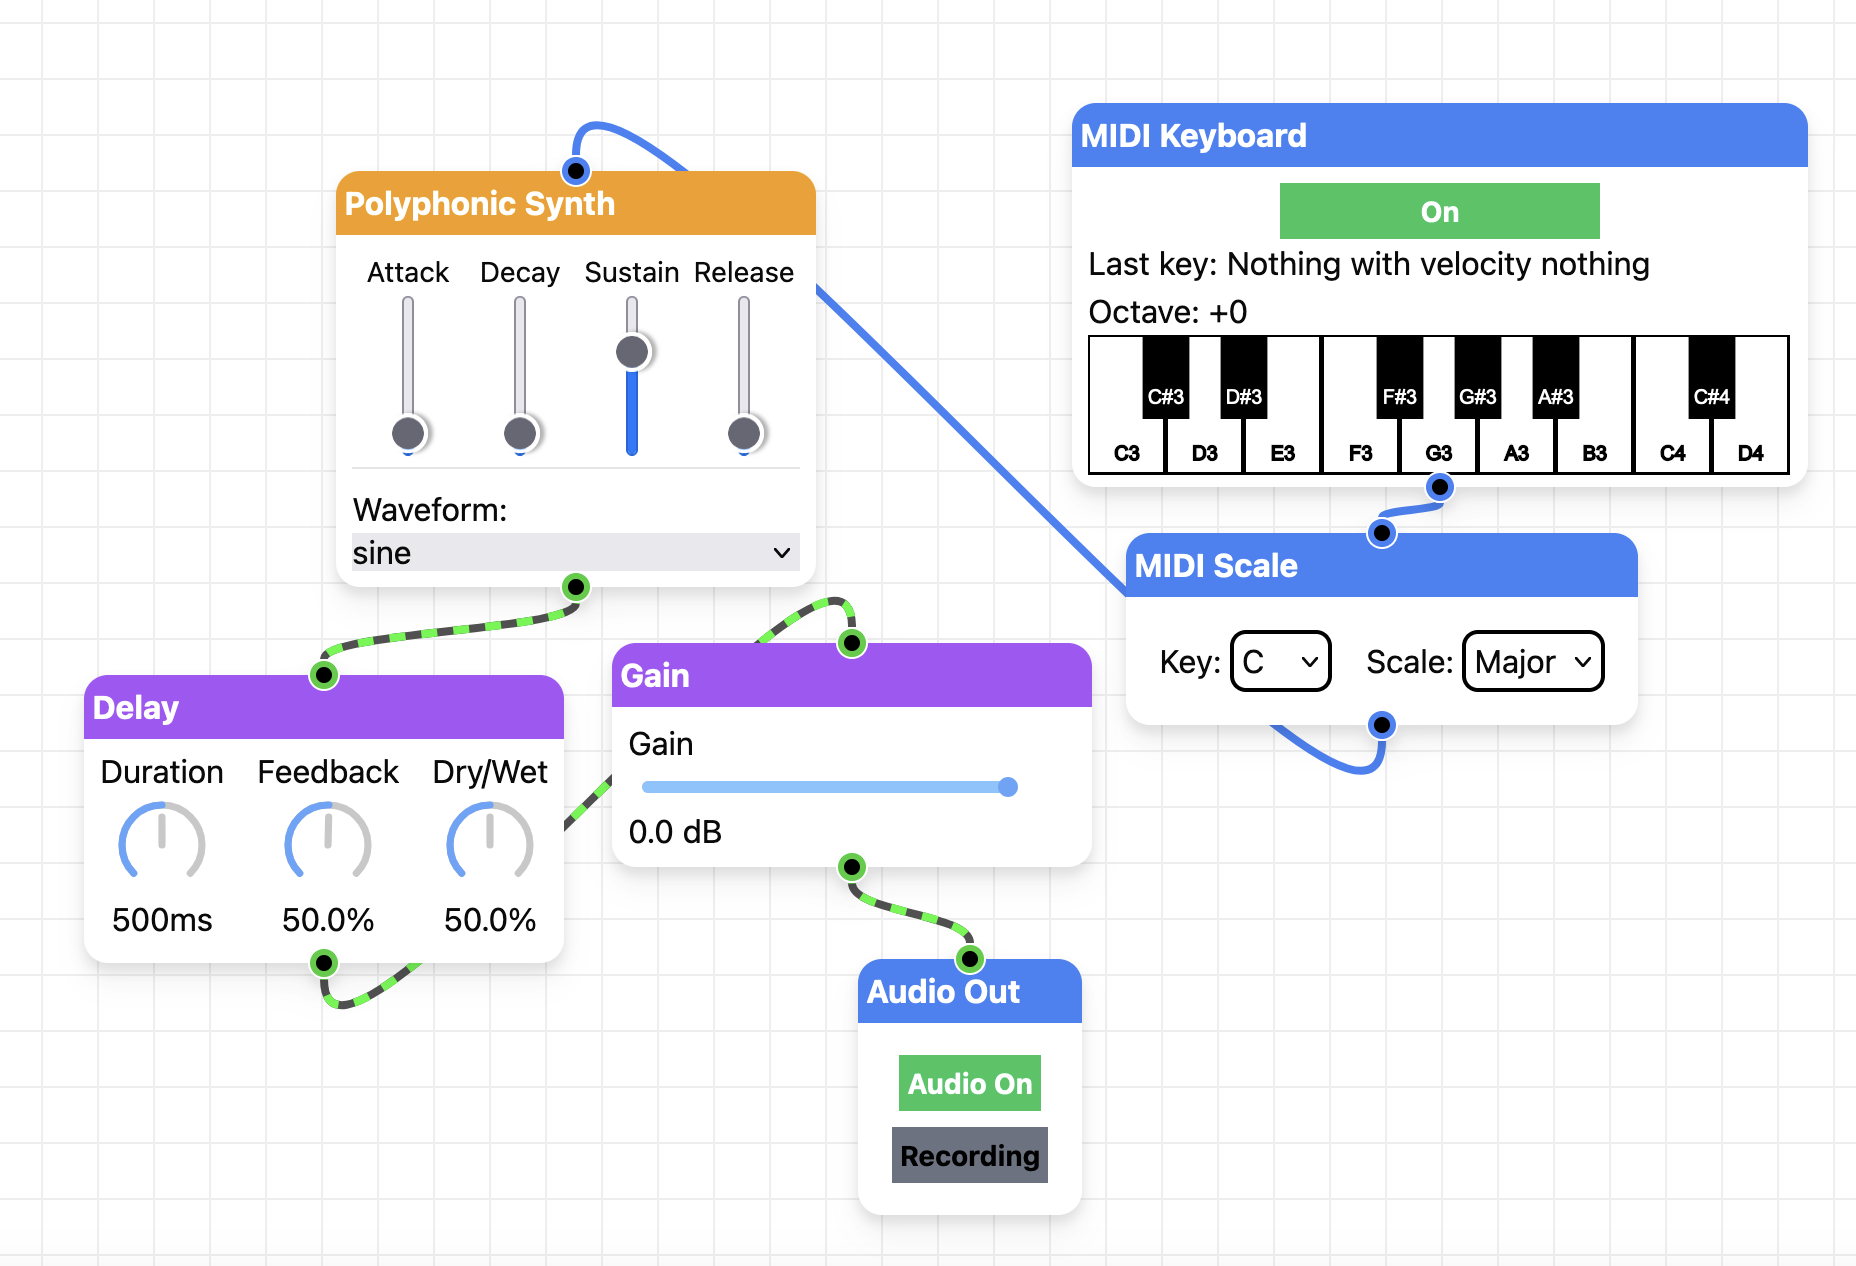
\includegraphics[width=0.45\textwidth]{images/nodeaa.png}
    \caption{Nodeaa's interface and a basic signal flow.}
    \label{fig:nodeaa}
\end{figure}

\section{Problem Statement}

The primary problem \textit{Nodeaa} addresses is the lack of accessible, cross-platform tools for real-time modular audio processing and dynamic routing. While traditional DAWs like Ableton Live and Logic Pro offer extensive features, they require significant system resources, installations, and are often prohibitively expensive. Similarly, tools like MaxMSP and Pure Data are powerful but can present steep learning curves, limiting their accessibility to users with advanced DSP programming knowledge. This creates a significant barrier for beginners, educators, and those without access to high-performance hardware or expensive software licenses. Table~\ref{tab:comparison} compares the features of traditional DAWs, modular tools, and Nodeaa.

\subsection{Accessibility Challenges in Audio Processing}

The accessibility of audio tools is constrained by both technical and financial factors. High-performance DAWs often require powerful hardware and advanced knowledge, placing them out of reach for many users. Educational institutions and hobbyists in resource-limited regions face additional hurdles due to the cost and complexity of these tools. This disparity hinders creativity and innovation by excluding a large portion of potential users who lack the means to experiment with digital audio.

\subsection{Democratizing Audio Tools Through the Web}

By leveraging the browser as a platform, \textit{Nodeaa} addresses these challenges head-on. Users can access \textit{Nodeaa} from any modern desktop device with a web browser, eliminating the need for installations or specialized hardware. This approach significantly reduces entry barriers and allows musicians, educators, and hobbyists to explore modular audio processing without requiring advanced technical expertise \cite{leyshon2014reformatted}. The web-based nature of \textit{Nodeaa} ensures cross-platform compatibility, reaching users regardless of their operating system or device specifications.

\begin{table*}[ht]
\centering
\caption{Comparison of Traditional DAWs, Modular Tools, and Nodeaa}
\label{tab:comparison}
\begin{tabular}{|l|l|l|l|}
\hline
\textbf{Feature/Aspect}                  & \textbf{Traditional DAWs}         & \textbf{Modular Tools (e.g., Max/MSP)} & \textbf{Nodeaa}        \\ \hline
\textbf{Platform Dependency}             & High                              & High                                   & Low                    \\ \hline
\textbf{Cost}                            & Expensive                         & Expensive (or limited free options)    & Free and Open Source   \\ \hline
\textbf{Installation Required}           & Yes                               & Yes                                    & No (Browser-Based)     \\ \hline
\textbf{Hardware Requirements}           & High                              & Moderate to High                       & Low                    \\ \hline
\textbf{Ease of Use for Beginners}       & Moderate                          & Low (Steep Learning Curve)             & High                   \\ \hline
\textbf{Flexibility and Customization}   & High                              & Very High                              & High                   \\ \hline
\textbf{Cross-Platform Accessibility}    & Limited (OS-Specific)             & Limited (OS-Specific)                  & Universal (Web-Based)  \\ \hline
\textbf{Real-Time Audio Processing}      & Yes                               & Yes                                    & Yes                    \\ \hline
\textbf{Community and Educational Use}   & Limited (Cost Barrier)            & Limited (Complexity Barrier)           & Broad                  \\ \hline
\textbf{Extensibility via Code or Nodes} & Limited (Plugins)                 & High                                   & High                   \\ \hline
\end{tabular}
\end{table*}

\section{Technical Background}

To understand the development and functionality of \textit{Nodeaa}, it is essential to detail the underlying technologies and concepts that enable it. \textit{Nodeaa} combines principles of modular audio processing, node-based dynamic routing, and modern web development frameworks. Below, we introduce the key technical foundations necessary for this project.

\subsection{WebAudio API}

The WebAudio API is a high-level JavaScript API for processing and synthesizing audio in web applications. It provides a graph-based model where audio processing is performed by connecting various \textit{AudioNodes}, such as sources, effects, and output nodes. Each \textit{AudioNode} represents a single processing module, and developers can dynamically create and route connections between nodes to build complex audio graphs \cite{smus2013web}. The API also supports features like real-time audio processing, spatial audio, and playback control, making it a robust tool for browser-based audio applications.

\subsection{Node-Based Interfaces}

Node-based interfaces represent data or processes as interconnected nodes in a visual graph \cite{burnett1995visual}. Each node performs a specific function, such as generating sound, applying an effect, or routing data. Users can intuitively connect nodes to define the flow of data or signals, enabling modular and flexible workflows. This pattern is widely used in audio programming environments such as MaxMSP, Pure Data, and VCV Rack, and \textit{Nodeaa} brings this approach to the browser.

\subsection{WebAssembly (Wasm)}

WebAssembly is a low-level binary instruction format designed for efficient execution in web browsers \cite{haas2017bringing}. It enables near-native performance for computationally intensive tasks by compiling code written in languages like C++ and Faust into a format that the browser can execute. In \textit{Nodeaa}, WebAssembly is used to load custom audio nodes compiled from Faust and RNBO code, allowing developers to extend the functionality of the WebAudio API with high-performance, user-defined modules.

\subsection{React and React Flow}

React is a popular JavaScript library for building user interfaces \cite{fedosejev2015react}. It enables developers to create reusable components that manage their own state, simplifying the development of complex web applications. React Flow is a library built on React for creating interactive node-based interfaces. It provides the core functionality needed for rendering, connecting, and managing nodes and edges in \textit{Nodeaa}, allowing users to visually construct and manipulate audio graphs.

\subsection{Audio Signal Flow}

Understanding audio signal flow is critical for working with \textit{Nodeaa}. Audio signals are continuous streams of data representing sound waves, which are processed in real time by connecting input, processing, and output nodes \cite{roads1996computer} \cite{wakefield2022generating}. For instance, in a simple setup, a microphone's audio input is routed to a delay effect node and then to the speakers. Signal processing involves modifying these streams through operations like filtering, amplification, and spatialization to achieve desired audio effects.

\subsection{Faust and RNBO}

Faust (Functional Audio Stream) and RNBO (a node-based language associated with MaxMSP) are key technologies enabling the features of \textit{Nodeaa}.

Faust is an open-source, domain-specific functional programming language for real-time audio signal processing. It allows developers to create DSP algorithms with a high-level syntax that can be compiled into multiple formats, including WebAssembly, making it an ideal choice for integrating custom audio nodes into browser-based platforms like \textit{Nodeaa} \cite{orlarey2009faust}.

Similarly, RNBO provides a low-level, node-based environment for designing audio processing and synthesis workflows. It supports exporting these workflows to WebAssembly, enabling seamless integration with web audio applications \cite{kilius2015web}.

By combining these technologies, \textit{Nodeaa} bridges the gap between traditional DAWs and web-based tools, offering a modular environment for sound processing directly in the browser. This integration highlights the potential of modern web technologies to deliver advanced audio synthesis and processing capabilities traditionally reserved for desktop applications.

\section{Prior Work}

The development of \textit{Nodeaa} draws heavily on concepts and techniques from existing tools and frameworks in digital audio processing, each contributing unique approaches to sound synthesis and manipulation.

\subsection{Faust in Digital Audio Processing}

Faust has established itself as a powerful functional programming language for real-time audio signal processing and synthesis. Its ability to compile high-level functional code into efficient low-level implementations makes it highly versatile, supporting deployment on platforms ranging from embedded systems to web applications \cite{orlarey2009faust}. Faust’s integration into \textit{Nodeaa} demonstrates how its modular, high-level syntax can be leveraged to create advanced audio effects and instruments tailored for modern web environments \cite{letz2017compiling, letz2015faust}.


\subsection{Max/MSP and Pure Data}

\begin{figure}[ht]
    \centering
    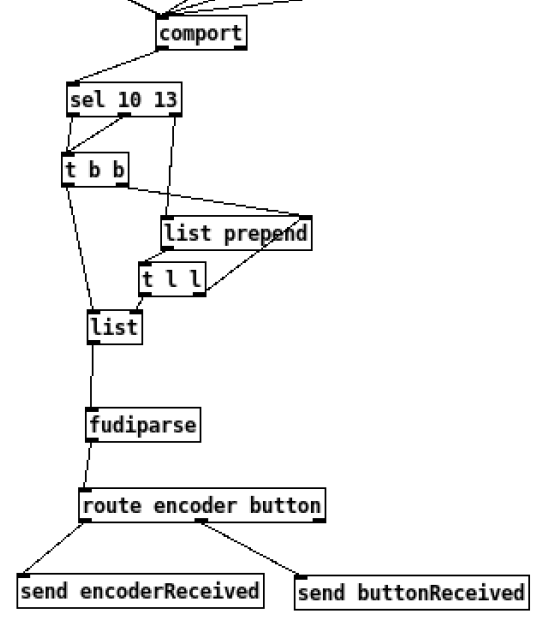
\includegraphics[width=0.2\textwidth]{images/puredata.png}
    \caption{An example DSP chain in Pure Data}
    \label{fig:puredata}
\end{figure}

Max/MSP and Pure Data (Pd) are visual programming environments that promote the creation of interactive multimedia applications \cite{puckette1996pure}. They employ a node-based interface where users connect objects representing different functions to design complex audio and visual processes. This modular approach provides significant flexibility and customization, enabling users to develop intricate signal processing chains and interactive installations. However, the depth of customization available can present a steep learning curve for newcomers, potentially limiting accessibility for those without prior experience in audio programming.

\subsection{Bitwig Studio's The Grid}

\begin{figure}[ht]
    \centering
    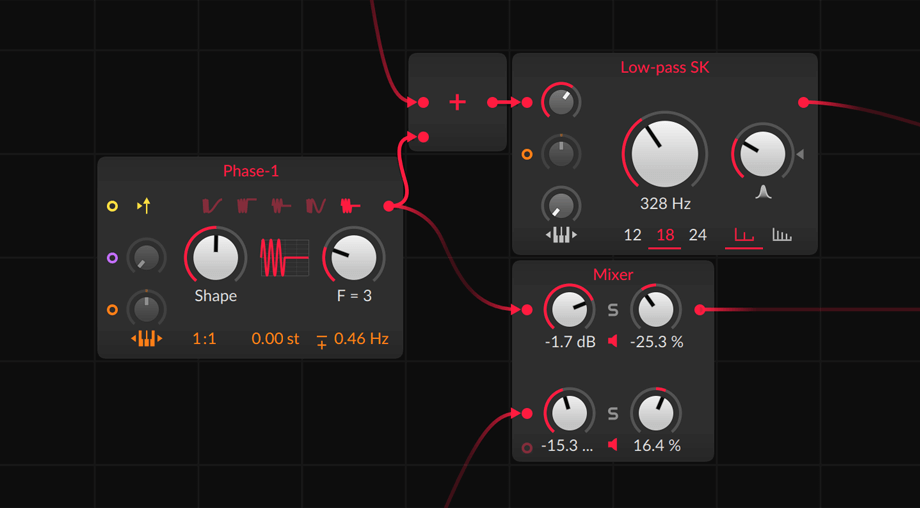
\includegraphics[width=0.4\textwidth]{images/thegrid.png}
    \caption{Another node based audio routing program, The Grid in Bitwig Studio}
    \label{fig:grid}
\end{figure}

Bitwig Studio's The Grid is a modular sound design environment integrated within the Bitwig digital audio workstation \cite{burt2023new}. It offers a high-level, guided interface for creating audio effects and instruments, emphasizing user-friendly interaction and a simple workflow. While The Grid simplifies the process of sound design, its high-level nature may impose certain limitations on the depth of customization and flexibility compared to more low-level programming environments like FAUST or Max/MSP.

\subsection{Influence on \textit{Nodeaa}}

The design and development of \textit{Nodeaa} are informed by the strengths and limitations of these existing tools. By integrating the flexibility of node-based audio routing, as exemplified by Max/MSP and Pure Data, with the accessibility of a browser-based platform, \textit{Nodeaa} aims to provide a balanced environment for both novice and experienced users. Additionally, by compiling FAUST code into WebAssembly (Wasm), \textit{Nodeaa} leverages efficient, low-level audio processing capabilities within the browser context, bridging the gap between high performance and user-friendly interaction.

\section{Methods}

\subsection{Project Structure and Development Workflow}
The development of \textit{Nodeaa} follows a streamlined Continuous Integration/Continuous Deployment (CI/CD) workflow utilizing GitHub Actions \cite{chandrasekara2021introduction}. This ensures that every change is automatically tested and deployed to the live site, enabling rapid iteration and consistent delivery. Each change is subjected to automated checks for performance and building before deployment. By eliminating manual deployment steps, the workflow reduces human error and speeds up the development cycle. This approach ensures that users consistently experience a reliable and up-to-date application.

\subsection{Integration of Faust and RNBO for Custom Audio Nodes}
A key component of \textit{Nodeaa}'s functionality is its ability to integrate custom audio nodes compiled from Faust and RNBO code \cite{kilius2015web} \cite{letz2017compiling} \cite{letz2015faust}. These nodes implement custom algorithms tailored for specific audio processing tasks, such as delays, synthesizers, and filters. The compilation process transforms the Faust and RNBO scripts into WebAssembly (WASM) modules, which are then added to the public directory of the web app for direct access by the browser. To enable user interaction with these modules, a TypeScript interface is created to manage their parameters dynamically, allowing seamless control and real-time adjustments. Additionally, an entry is added to the master JSON file to define the node's metadata, including its name, default parameters, audio type, public URL, and version. This modular approach simplifies the addition of new nodes and ensures compatibility within the existing ecosystem.

\subsection{Graphical Interface and Node Management}

The node-based interface is built using React Flow, which is extensively customized to enhance its functionality and usability. React Flow provides a robust foundation for visualizing and managing node connections, but \textit{Nodeaa} extends its capabilities by incorporating state persistence through Zustand. This allows users to save and reload projects seamlessly, preserving all node configurations and connections. Visual clarity is a priority, and connection wires are color-coded to indicate the type of data being transmitted: green-striped for audio, blue for MIDI, and grey for general data. Such visual distinctions help users quickly understand the routing within their projects. While alternative libraries were evaluated, they often relied on \texttt{<canvas>} elements, which would have shifted focus to graphics programming and increased complexity. By leveraging React Flow, \textit{Nodeaa} maintains an intuitive interface that prioritizes functionality and accessibility.

\begin{figure}[ht]
    \centering
    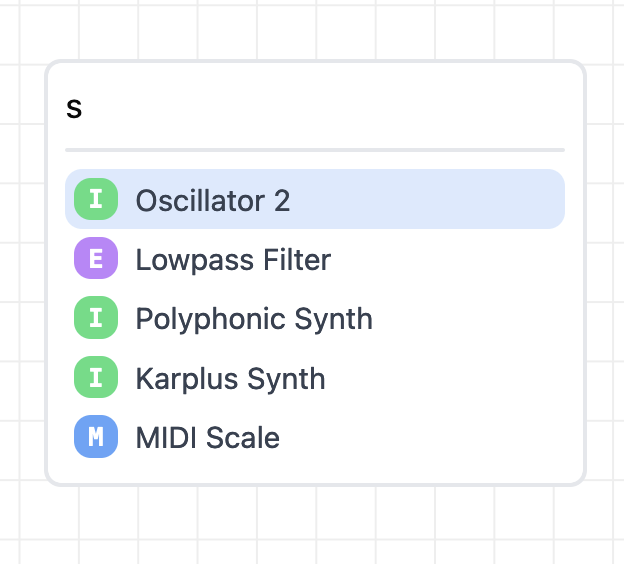
\includegraphics[width=0.28\textwidth]{images/nodeaacreator.png}
    \caption{The node creator created by pressing "n" on the keyboard. Allows users to quickly create nodes by typing and getting instant results.}
    \label{fig:nodeaacreator}
\end{figure}

\subsection{Latency Management and Real-Time Performance}
Low latency is critical for live audio performance, and \textit{Nodeaa} is designed to achieve this without overburdening the system. The application introduces slight latencies (~1ms) to clear the audio thread and prevent overloading, ensuring smooth playback even under demanding conditions \cite{buffa2024can}. Each node operates independently in the audio thread, leveraging the WebAudio API to manage audio connections and processing \cite{kleimola2015web}. This decentralized state management architecture minimizes inter-node communication overhead, allowing the system to scale efficiently. Additionally, the application prioritizes real-time audio performance by optimizing its scheduling, ensuring that user actions translate to immediate auditory feedback without noticeable delays.

\subsection{Design Decisions}
The design of \textit{Nodeaa} draws inspiration from industry-standard audio software such as Ableton Live and MaxMSP. Key user interface elements, including knobs and sliders, are modeled to emulate the tactile experience of professional audio equipment \cite{gomez2011usage}. These abstract components are designed for both aesthetic appeal and functional clarity, enhancing the overall user experience for users. The connection process between nodes mimics MaxMSP's intuitive drag-and-drop system, simplifying the creation of complex audio routing configurations. By adopting these proven design principles, \textit{Nodeaa} lowers the learning curve for new users while maintaining the flexibility and power required by experienced professionals.

\begin{figure}[ht]
    \centering
    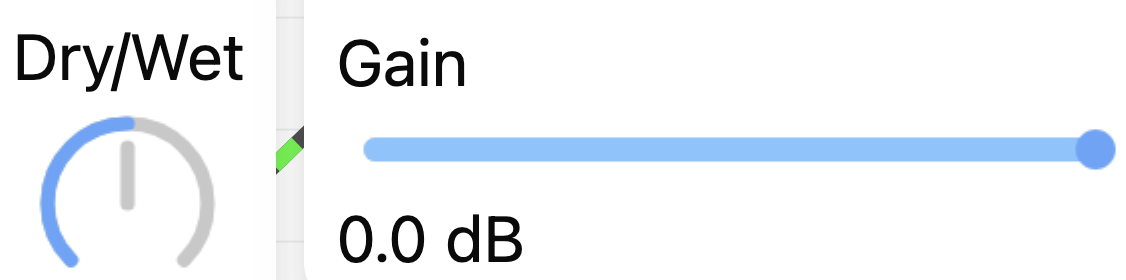
\includegraphics[width=0.4\textwidth]{images/nodeaaui.png}
    \caption{Example of two custom Nodeaa interface components, Knob and Slider.}
    \label{fig:nodeaaui}
\end{figure}

\subsection{Developer Tools and Components}

During development, \textit{Nodeaa} introduced a selection of tools to support extensibility and customization. These tools include the aforementioned versatile and abstract UI components such as knobs, sliders, and number boxes, all created using p5.js canvas elements. By optimizing these elements to redraw only during user interaction, the project achieves efficient performance while maintaining visual fidelity. These modular components can be easily integrated into custom nodes or applications, providing developers with flexible building blocks for their projects.

The project also implemented foundational components for creating node shapes, such as a container and a draggable title bar, allowing for the design of cohesive and interactive nodes. Custom React hooks were developed to listen for specific event data, including MIDI input, enabling dynamic and responsive audio workflows with minimal boilerplate code. While the tools are limited due to time constraints, they establish a foundation for future expansion.

\subsection{Context-Aware Information Display}

Inspired by Ableton Live \cite{robinson2014ableton}, \textit{Nodeaa} incorporates a dynamic information box located in the bottom left corner of the interface. This feature provides real-time contextual documentation about the parameter or device that the user’s mouse is currently hovering over. For example, hovering over a knob displays its function, parent device, and an explanation of its effect, while hovering over a device provides a brief description of its overall purpose and usage.

This design choice ensures that users have immediate access to relevant information without disrupting their workflow. Beginners benefit from reduced reliance on external documentation, while experienced users can quickly reference details about less frequently used features. By embedding this intuitive guidance directly into the interface, \textit{Nodeaa} fosters a more seamless and efficient user experience, aligning with its goal of being accessible to users of all skill levels.

\begin{figure}[ht]
    \centering
    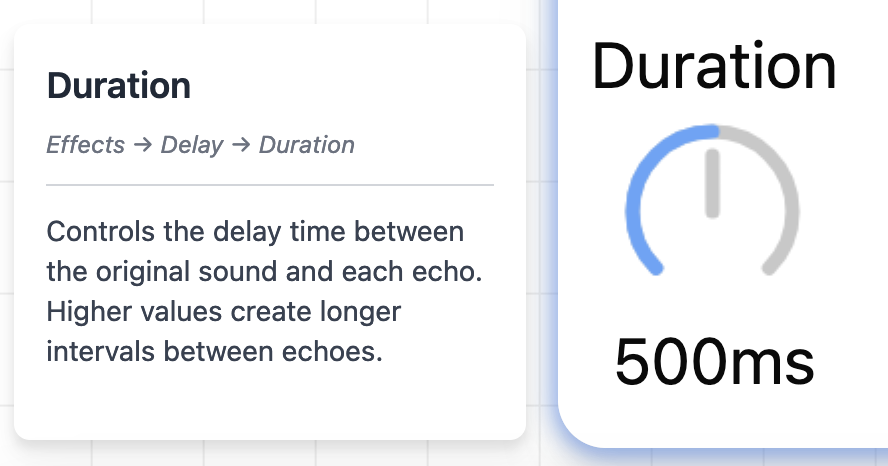
\includegraphics[width=0.4\textwidth]{images/nodeaainfo.png}
    \caption{The info panel seen here showing the description for the delay duration knob on the delay effect.}
    \label{fig:nodeaainfo}
\end{figure}

\subsection{Limitations and Alternatives}
While the browser-based implementation of \textit{Nodeaa} addresses accessibility and ease of use, it is not without limitations. JavaScript's single-threaded nature imposes constraints on performance \cite{verdu2015performance}, particularly when handling large projects with over 1,000 nodes \cite{chkec2019performance}. Such scenarios can introduce graphics related paint lag, and tasks like audio parameter updates may require more time compared to native C++ desktop applications. A desktop application was considered as an alternative, but this approach would have negated the primary goal of eliminating installation barriers and providing a truly cross-platform solution. Despite these challenges, \textit{Nodeaa} remains a highly capable tool for live audio performance and modular sound processing, offering a unique blend of accessibility and functionality.

\section{Evaluation Metrics}

The success of \textit{Nodeaa} is evaluated based on its ability to deliver real-time, low-latency audio processing, an intuitive user experience for both beginners and advanced users, and compatibility across major desktop browsers. Metrics were chosen to measure the system’s performance, usability, and creative potential, ensuring the site meets the needs of a broad user base.

\subsection{Performance Metrics}
Real-time performance was assessed by observing audio playback quality and responsiveness. Key indicators included the absence of audio glitches, such as clicks and pops, and smooth operation without perceptible lag, even under complex routing scenarios. These metrics were tested under varying levels of system load to ensure the tool remained stable and responsive in real-world use cases. Additionally, the performance of custom audio nodes, compiled from Faust and RNBO to WebAssembly, was evaluated to confirm that they integrated seamlessly into the broader audio graph. Browser compatibility was validated across major desktop browsers, including Chrome, Firefox, and Brave, ensuring users could reliably access the application regardless of their preferred platform.

\subsection{Usability and Accessibility}
Usability was evaluated through two rounds of user testing with two different versions of Nodeaa. Feedback was gathered via structured forms focusing on ease of use, clarity of the interface, and the tool’s ability to inspire creativity. During testing, users were tasked with completing specific workflows, such as routing a microphone input through an effect node and recording the output, to assess the intuitiveness of the interface. Metrics included the time required to understand and complete these tasks, the clarity of visual feedback provided by the node-based interface, and subjective ratings of the tool’s overall usability. Additionally, the design was tested for accessibility features, ensuring that users with different levels of technical expertise could engage with the software effectively.

\subsection{Creative Potential}
To assess creative potential, users were asked whether \textit{Nodeaa} supported their ability to create music or perform live. Specific feedback was requested on the extent to which the current feature set enabled meaningful exploration and experimentation. The metrics also included evaluations of the variety and flexibility of available nodes, as well as the ease of combining them to achieve unique audio effects. Insights were drawn from user feedback to identify potential areas for future feature development, such as additional node types or advanced customization options. Importantly, the evaluation aimed to determine whether users found the tool inspiring and versatile enough to include in their personal or professional projects.

\subsection{Exclusions}
While mobile compatibility was considered, it was ultimately excluded as a primary metric due to the project’s focus on desktop environments. Mobile platforms often present unique challenges \cite{clauhs2022daw}, such as reduced processing power and limited screen real estate, which were beyond the scope of this project. Similarly, analysis with existing DAWs was de-prioritized in favor of metrics that evaluate \textit{Nodeaa}'s standalone utility. This decision reflects the focus on the unique contributions of \textit{Nodeaa}, particularly its browser-based architecture and node-based interface, rather than positioning it as a direct competitor to traditional DAWs.

These metrics provide a comprehensive framework for determining the success of \textit{Nodeaa} in meeting its goals and addressing the identified problem.

\section{Results and Discussion}

The results of the evaluation indicate that \textit{Nodeaa} has successfully addressed many of its intended goals. By analyzing user feedback and metrics, the tool has demonstrated strong performance, usability, and creative potential. Below, the key findings are summarized and discussed in the context of the project’s objectives.

\subsection{Performance Metrics}
One of the primary objectives of \textit{Nodeaa} was to ensure real-time, low-latency audio performance suitable for live use. According to user responses, \textit{Nodeaa} met this goal effectively:
\begin{itemize}
    \item 100\% of users reported no audio glitches such as clicks or pops during their sessions.
    \item 89.5\% of users found audio playback to be consistently responsive, with low latency. Only 10.5\% noted occasional lag, primarily when interacting with the interface.
    \item The application remained stable in complex routing scenarios, as confirmed by 100\% of users.
\end{itemize}
While some lag was reported during interface interactions \cite{chkec2019performance}, the system’s core audio performance was robust. Issues in Safari were noted by 15.8\% of users, suggesting the need for further optimization for non-Chromium-based browsers.

\subsection{Usability and Accessibility}
\begin{figure}[ht]
    \centering
    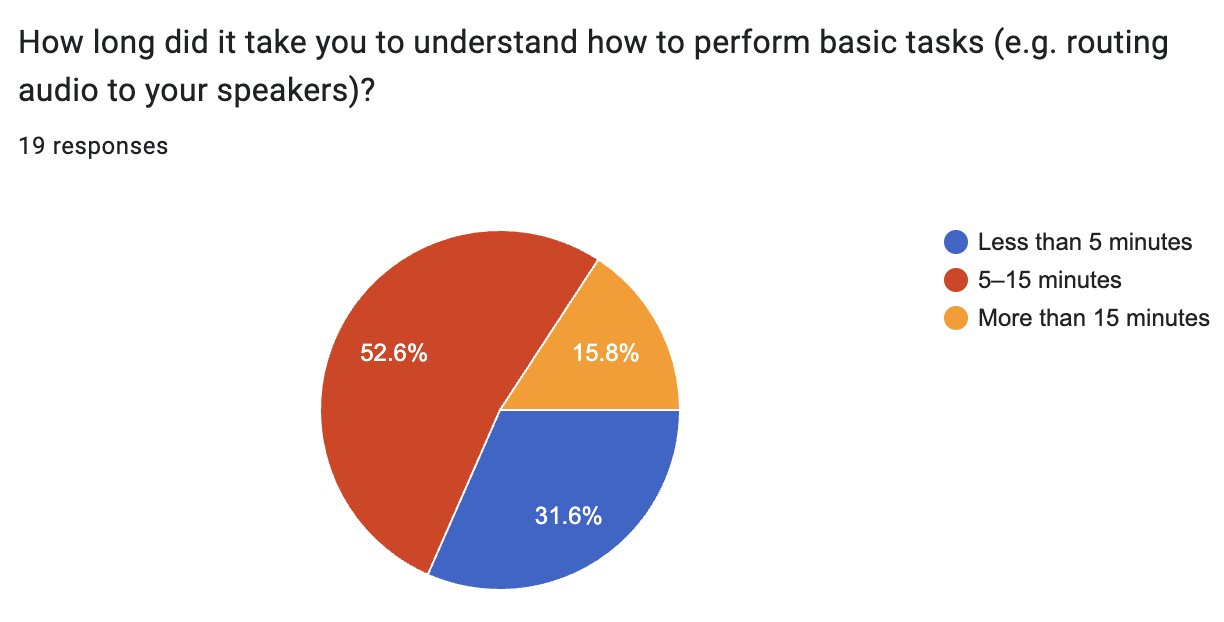
\includegraphics[width=0.46\textwidth]{images/surveytime.png}
    \caption{A graph showing the responses to time spent learning Nodeaa for the first time.}
    \label{fig:surveytime}
\end{figure}
Another critical goal was to create a tool that is accessible to both beginners and advanced users. Feedback on the interface highlighted both strengths and areas for improvement:
\begin{itemize}
    \item 42.1\% of users rated the interface as a 3 out of 5 for intuitiveness, while 42.1\% gave it a 4, and 15.8\% rated it a 5. This indicates a generally positive reception but also room for refinement.
    \item Most users (52.6\%) were able to understand basic tasks within 5–15 minutes, demonstrating the tool’s approachability. However, 15.8\% required more than 15 minutes.
    \item 94.7\% of users agreed that the interface provided clear feedback, though minor issues were reported, such as a bug requiring multiple clicks to delete a node and the ability to create feedback loops by connecting nodes to themselves.
    \item 57.9\% of users encountered barriers related to their expertise. Common challenges included unfamiliar terms (e.g., "karplus") and confusion about specific concepts like MIDI devices. Suggestions for tutorial videos or in-app guidance were frequently mentioned.
\end{itemize}
These findings emphasize the need for enhanced on-boarding resources and clearer terminology to improve accessibility for beginners.

\begin{figure}[ht]
    \centering
    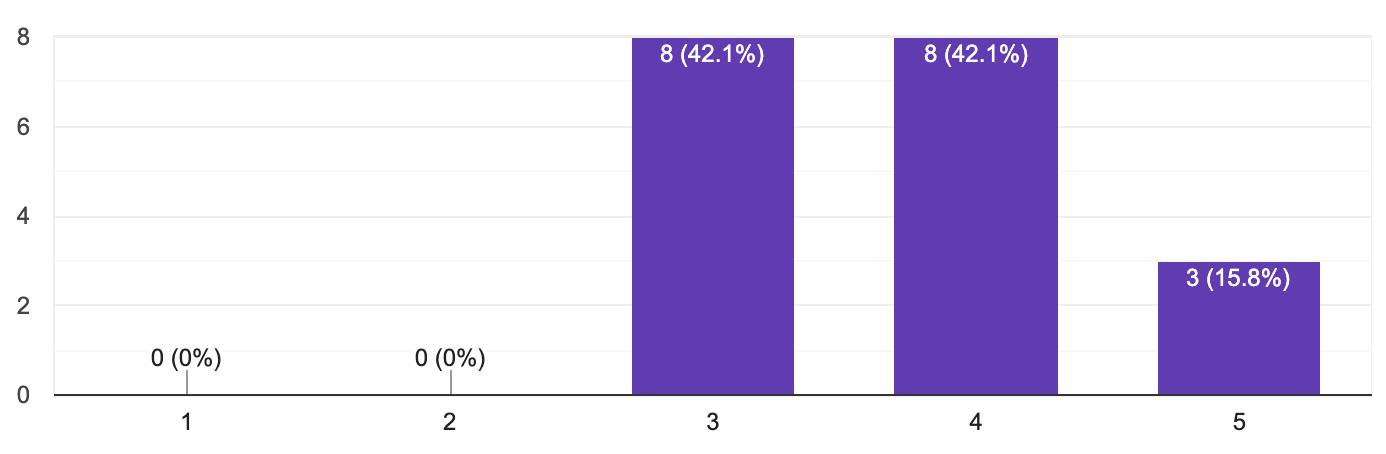
\includegraphics[width=0.46\textwidth]{images/surveyinterface.png}
    \caption{A graph showing the responses to "How intuitive did you find the node-based interface?" on a scale of 1-5 (5 being very intuitive).}
    \label{fig:surveyinterface}
\end{figure}

\subsection{Creative Potential}
\textit{Nodeaa} excelled in enabling users to experiment and create:
\begin{itemize}
    \item 100\% of users felt they could experiment easily with the current feature set.
    \item 68.4\% of users found the available nodes to somewhat support their creative goals, while 31.6\% felt they fully supported them. No users reported dissatisfaction.
    \item 94.7\% of users envisioned using \textit{Nodeaa} in future projects, underscoring its potential as a practical and inspiring tool.
\end{itemize}
User feedback frequently highlighted the desire for additional effects, instruments, and advanced nodes to expand the creative possibilities.

\begin{figure}[ht]
    \centering
    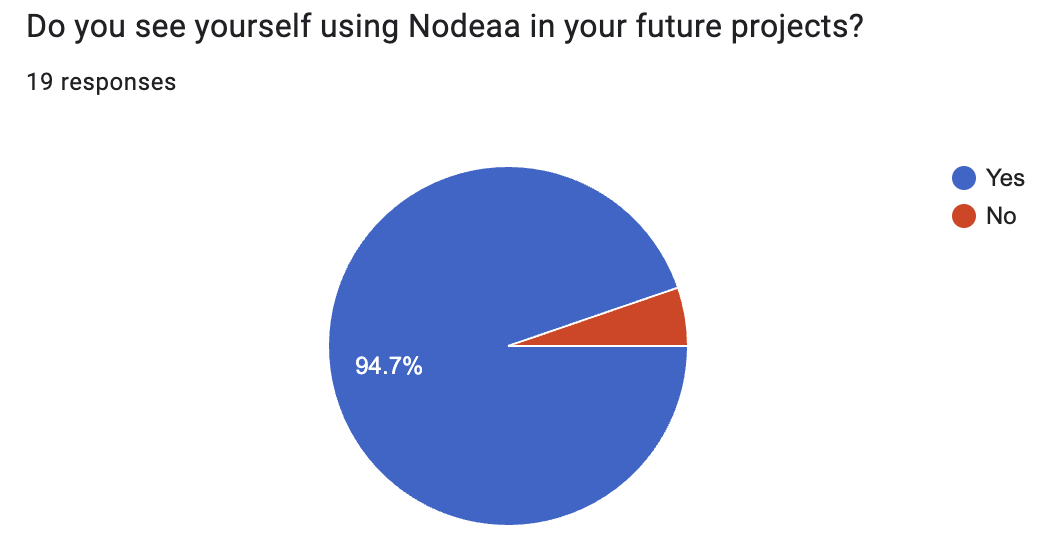
\includegraphics[width=0.46\textwidth]{images/surveyuseagain.png}
    \caption{A graph showing the responses to using Nodeaa in future projects.}
    \label{fig:surveyuseagain}
\end{figure}

\subsection{Caveats and Alternate Explanations}
While the results are largely positive, some caveats should be considered:
\begin{itemize}
    \item The sample size of advanced users was limited (5.3\%), which may underrepresent the needs of highly experienced users.
    \item Browser compatibility issues in Safari indicate that further testing and optimization are necessary to ensure cross-browser functionality.
    \item The reported usability barriers, while expected for a modular tool, suggest a need for improved documentation and in-app tutorials to bridge the gap for novice users.
\end{itemize}

\begin{figure}[ht]
    \centering
    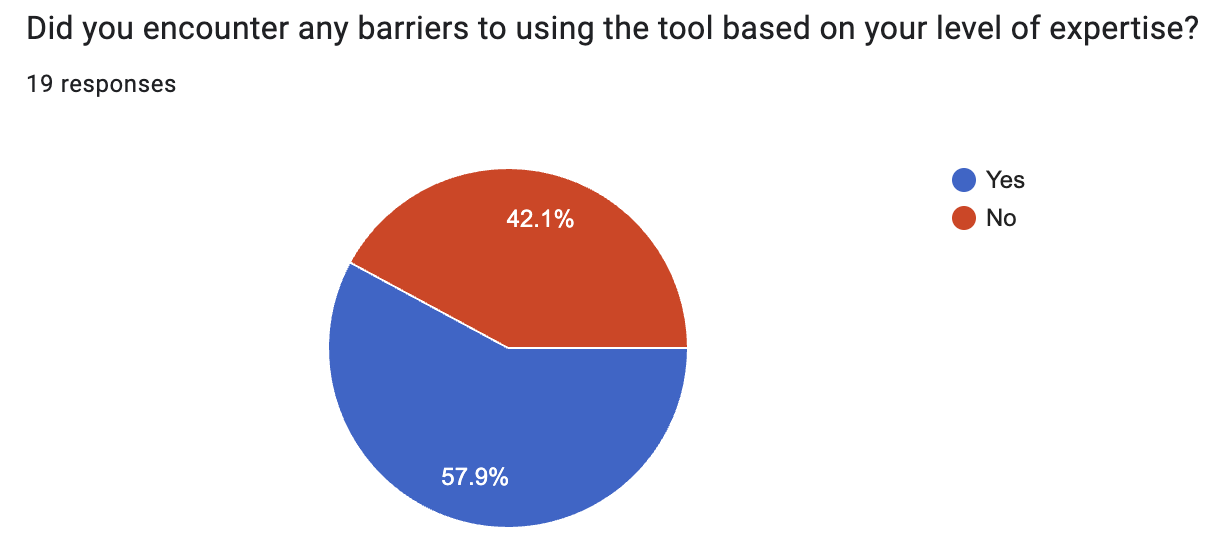
\includegraphics[width=0.46\textwidth]{images/surveybarriers.png}
    \caption{A graph showing the responses to barrier based on skill level.}
    \label{fig:surveybarriers}
\end{figure}

\subsection{Summary}
Overall, \textit{Nodeaa} successfully meets its primary objectives of delivering real-time, low-latency audio performance and fostering creativity through a browser-based platform. By addressing the identified usability challenges and expanding the feature set, \textit{Nodeaa} has the potential to further solidify its role as an innovative and accessible digital audio workstation.

The raw data and user feedback collected during testing are available in the project repository for further reference: \url{https://github.com/a200xeaf/nodeaa2}.

\section{Ethical Considerations}

Developing and deploying \textit{Nodeaa} involves several ethical considerations, both technological and biological. These issues highlight the responsibility of developers to create tools that are safe and equitable.

\subsection{Hearing Safety and Equipment Protection}
One of the primary ethical concerns in audio software development is ensuring user safety by preventing excessively loud sounds, clicks, or pops, which can damage both hearing and audio equipment \cite{zhao2010music} \cite{pienkowski2021loud}. \textit{Nodeaa} mitigates these risks by:
\begin{itemize}
    \item Ensuring that audio nodes are designed with safeguards against extreme volume levels, such as default gain limits.
    \item Feedback loop prevention in the audio graph.
    \item Testing to ensure that the custom nodes real-time processing does not introduce unintended audio artifacts under normal operation.
    \item A clipping limiter placed on the output to prevent audio that exceeds -1.0 - 1.0 amplitude range.
\end{itemize}
Future iterations of \textit{Nodeaa} will explore real-time peak monitoring to further enhance safety measures and smoother output limiting options.

\subsection{Intellectual Property and Copyright Concerns}
As \textit{Nodeaa} evolves, particularly with the potential for future versions to allow sharing, uploading, or recording of user-generated projects, intellectual property (IP) and copyright issues may arise. For example:
\begin{itemize}
    \item Users may inadvertently or intentionally include copyrighted audio samples or MIDI sequences in their projects.
    \item Distributed projects could be used to bypass copyright protections, raising potential legal and ethical challenges.
\end{itemize}
To address these concerns, the development roadmap includes plans for:
\begin{itemize}
    \item Implementing basic content analysis tools \cite{acoustid} that identify copyrighted material before projects are shared or distributed.
    \item Providing clear terms of use that emphasize users’ responsibility for ensuring compliance with copyright laws.
\end{itemize}
These measures aim to balance the creative freedom \textit{Nodeaa} offers with a commitment to respecting the rights of content creators.

\subsection{Accessibility and Inclusivity}
While \textit{Nodeaa} strives to be an accessible tool for users across skill levels, ethical considerations regarding diversity and inclusivity remain:
\begin{itemize}
    \item The interface and terminology may pose barriers to non-technical users or individuals unfamiliar with modular audio systems. To address this, future updates will begin work on localized language.
    \item Browser-based tools require reliable internet and modern hardware, which may inadvertently exclude users in regions with limited technological access. This highlights the need for further exploration of offline functionality and optimization for lower-spec devices.
\end{itemize}

\subsection{Conclusion}
Ethical considerations are important to the development of \textit{Nodeaa}. By addressing safety, IP concerns, inclusivity, and safety, the site aims to create a responsible and impactful tool that is useful to users without compromising ethical standards. Future development will continue to prioritize these concerns, ensuring that \textit{Nodeaa} remains a safe platform for creative expression.

\appendix
\section{Replication Instructions}

To replicate and use \textit{Nodeaa}, follow these instructions carefully. These steps ensure compatibility and reproducibility of the project setup.

\subsection{Prerequisites}
Before starting, ensure that the following software is installed:
\begin{itemize}
    \item Node.js (version 16.0.0 or higher)
    \item npm (version 7.0.0 or higher)
    \item A modern web browser (such as Google Chrome or Mozilla Firefox)
\end{itemize}
For consistent results, it is recommended to use the specified versions or later.

\subsection{Cloning the Repository}

Begin by cloning the project repository: \texttt{git clone https://github.com/a200xeaf/nodeaa2.git} and navigate to the directory using \texttt{cd nodeaa2}.

\subsection{Installing Dependencies}

Install the necessary packages using npm:
\begin{verbatim}
npm install
\end{verbatim}
This command will fetch and install all dependencies specified in the \texttt{package.json} file. Ensure that your internet connection is stable during this step.

\subsection{Running the Development Server}

Start the development server to run \textit{Nodeaa} locally:
\begin{verbatim}
npm run dev
\end{verbatim}
Open your browser and navigate to \url{http://localhost:5173} to access the application.

\subsection{Building for Production}

To create an optimized build for production, execute the following command:
\begin{verbatim}
npm run build
\end{verbatim}
The production-ready files will be placed in the \texttt{dist} directory.

\subsection{Previewing the Production Build}

To locally preview the production build, use the command:
\begin{verbatim}
npm run preview
\end{verbatim}
This will serve the application using the optimized build.

\subsection{Dependencies and Future-Proofing}

The project uses the following major dependencies:
\begin{itemize}
    \item React (version 18.0 or higher)
    \item TypeScript (version 5.0 or higher)
    \item Vite (version 5.0 or higher)
    \item RNBO (version 1.3.2 or higher)
    \item faustwasm (version 0.6.4 or higher)
\end{itemize}
For future-proofing, regularly update dependencies using \texttt{npm update}, but ensure that changes do not introduce breaking issues. Locking dependency versions in the \texttt{package.json} file helps maintain consistency.

\subsection{Survey Results and Documentation}

The repository includes the following additional files for reference:
\begin{itemize}
    \item \texttt{LATEXSOURCE/document.tex}: The full LaTeX source of this project paper.
    \item \texttt{SURVEYRESULTS/}: A folder containing raw survey data.
    \item \texttt{LICENSE}: The project license (AGPL v3).
\end{itemize}

\subsection{Contact for Issues}

For any issues or questions, consult the project repository's \texttt{README.md} or open an issue on the GitHub repository \url{https://github.com/a200xeaf/nodeaa2}.

\section{Code Architecture Overview}

This section provides an overview of \textit{Nodeaa}'s code architecture and instructions for extending the project, with a focus on adding new nodes and utilizing core features such as the store and audio engine.

\subsection{Folder Structure}
The project is organized as follows:
\begin{itemize}
    \item \texttt{src/engine}: Contains the core logic for the application, including \texttt{audio.ts}, which serves as the main engine for audio processing, and \texttt{store.ts}, which manages global application state using a reactive store architecture.
    \item \texttt{src/nodes}: Contains all node types grouped by their category (e.g., MIDI, Audio, Data).
    \item \texttt{public/nodes}: Stores precompiled WebAssembly (Wasm) and metadata files for Faust and RNBO nodes.
    \item \texttt{src/ui}: Houses reusable UI components such as sliders, knobs, and containers.
\end{itemize}
These folders work together to support the modular and extensible nature of \textit{Nodeaa}.

\subsection{Adding a New Node}
Adding a new node to \textit{Nodeaa} involves the following steps:

\subsubsection{Step 1: Compile to Wasm (If Applicable)}
If your node uses Faust or RNBO, compile your source to WebAssembly (Wasm):
\begin{itemize}
    \item For Faust, ensure the output includes \texttt{dsp-module.wasm} and \texttt{dsp-module.json}.
    \item For RNBO, include \texttt{(name).export.json} and \texttt{dependencies.json}.
    \item Place these files into a new folder under \texttt{public/nodes/}. Do not rename the files.
    \item Skip this step if creating non-audio nodes, such as MIDI devices.
\end{itemize}

\subsubsection{Step 2: Create the Node Component}
Create a new folder under \texttt{src/nodes/(type)/} and add a \texttt{.tsx} file representing the visual and functional implementation of the node.
\begin{itemize}
    \item Use \texttt{FC\textless{}NodeProps\textgreater{}} or \texttt{FC\textless{}NodeProps\textless{}YourNodeType\textgreater{}\textgreater{}} to define the component if it stores data.
    \item Define the node's data structure. For example:
\begin{lstlisting}
type MidiInNodeData = {
    midiin_device: string;
};

type MidiInNodeType = Node<MidiInNodeData, 'midiInNode'>;
\end{lstlisting}
    \item Use hooks like \texttt{useNodeStore} to update node parameters:
\begin{lstlisting}
const updateNode = useNodeStore((state) => state.updateNode);
// Usage: updateNode(id, { key: value });
\end{lstlisting}
    \item Define inlets and outlets with \texttt{\textless{}Handle /\textgreater{}}, referencing React Flow documentation for options.
\end{itemize}

\subsubsection{Step 3: Update the Master JSON File}
Add an entry for the new node to \texttt{nodes.json} using the following interface (Note: \texttt{"type": "name"} inside \texttt{"audioNodeParams"} should match the folder name in the public/nodes directory):
\begin{lstlisting}
export interface NodeConfig {
    nodeName: string;
    idPrefix: string;
    realName: string;
    defaultData: Record<string, unknown>;
    audioNodeParams?: {
        engine: "faust" | "rnbo";
        type: string;
        voices?: number;
    };
    hasAudio: boolean;
    audioType?: "instrument" | "effect";
    version: string;
};
\end{lstlisting}
For example:
\begin{lstlisting}
"faustGainNode": {
    "nodeName": "faustGainNode",
    "idPrefix": "",
    "realName": "Gain",
    "defaultData": { "faustgain_Gain": 1 },
    "audioNodeParams": { "engine": "faust", "type": "faustgain" },
    "hasAudio": true,
    "audioType": "effect",
    "version": "1.0.0"
},
\end{lstlisting}

\subsubsection{Step 4: Register the Node and Add Documentation}
\begin{itemize}
    \item Add the node to \texttt{nodeTypes} in \texttt{App.tsx}.
    \item Optionally, add hover-over documentation by updating \texttt{info-map.ts}:
\begin{lstlisting}
["midiInNode-check", {
    name: "Check Midi",
    parent: "MIDI In",
    type: "MIDI",
    description: "Checks for connected MIDI devices. Requires browser permission to work."
}]
\end{lstlisting}
    Use the \texttt{data-info-panel-id} attribute in your component for integration.
\end{itemize}

\subsection{UI Components and Hooks}
\textit{Nodeaa} provides several reusable components to streamline development:
\begin{itemize}
    \item \texttt{\textless{}Knob /\textgreater{}}, \texttt{\textless{}Numbox /\textgreater{}}, \texttt{\textless{}Slider /\textgreater{}}, \texttt{\textless{}PianoKeyboard /\textgreater{}}: Prebuilt UI elements for user interaction.
    \item \texttt{\textless{}NodeaaContainer /\textgreater{}}, \texttt{\textless{}NodeaaHeader /\textgreater{}}: Structural components for nodes.
    \end{itemize}
Custom hooks available include:
\begin{itemize}
    \item \texttt{useMidiNoteTracker}: Tracks active MIDI notes and processes MIDI events.
    \item \texttt{useEmitterSubscriptions}: Handles event subscriptions for connections.
\end{itemize}

These tools simplify extending the application and integrating new features seamlessly.

\printbibliography

\end{document}
